
\documentclass[10pt, a4paper]{article}

\usepackage[a4paper]{geometry}
\usepackage[utf8]{inputenc}
%\geometry{landscape} % Activate for for rotated page geometry
\usepackage{graphicx}
\usepackage{amssymb}
\usepackage{amsmath}
%\usepackage{epstopdf}
\usepackage{hyperref}
\usepackage{amsfonts}
%\usepackage{mathabx}
%\usepackage{topcapt}
\usepackage{listings}
\usepackage{color}
\usepackage{tikz}
\usepackage{graphicx}
\usepackage[margin=0.7cm]{caption}
\usepackage{subcaption}
\DeclareGraphicsExtensions{.pdf,.png,.jpg}


\begin{document}

\title{Obligatory Excercise 1 2014\\
\normalsize TMA4275 - Lifetime analysis\\
			NTNU}
\author{10057}
\date{\today}

\begin{titlepage}
\maketitle
\thispagestyle{empty}
\end{titlepage}

\section*{a)}
The Kaplan-Meier estimator is $ \hat{R}_1(t) = \prod \limits_{T_{1_i} \leq t} \frac{n_i-d_i}{n_i} $ where $ n_i $ is the number of units at risk, and $ d_i $ is the number of unit failing at time $t_i$, $ n_i = n_{i-1}-d_{i-1}-c_{i-1} $ where $ c_i $ is the censoring at time $T_i$.
The given values together with the formula gives the values in table \ref{r1hatt}.
\begin{center}
\begin{table}[h!]
\centering
\begin{tabular}{ c l c r }
& & & \\
time & expression & & value \\ & & \\
23 &  $ \frac{13-1}{13} $ & = & $ 0.9231 $\\ & & \\
47 &  $ \frac{13-1}{13}\cdot\frac{12-1}{12} $ & = & $ 0.8461 $\\ & & \\
69 &  $ \frac{13-1}{13}\cdot\frac{12-1}{12}\cdot\frac{11-1}{11} $ & = & $ 0.7692$ \\ & & \\
148 &  $ \frac{13-1}{13}\cdot\frac{12-1}{12}\cdot\frac{11-1}{11}\cdot\frac{6-1}{6} $ & = & $0.6410$ \\ & & \\
181 &  $ \frac{13-1}{13}\cdot\frac{12-1}{12}\cdot\frac{11-1}{11}\cdot\frac{6-1}{6}\cdot\frac{5-1}{5} $ & = & $ 0.5128 $\\
   & & \\

\end{tabular}
\caption{Table with survival probability for the negatively stained group.}
\label{r1hatt}
\end{table}
\end{center}
As we can see from the table above, the quantile for $t_{0.75}$ is approximate 69, but because of censoring there is not a good estimate for the $ t_{0.25}$ quantile. The median is also not possible to find because of the lack of $t_{0.25}$ quantile value.\\ 

Greenwoods formula is for standard error is $$\widehat{SD(\hat{R}_1(t))}= \sqrt{ \widehat{  \text{var}( \hat{R} (t))} }=  \hat{R}(t)  \cdot \sqrt{ \sum \limits_{T_{1_i} \leq t} \frac{d_i}{n_i (n_i-d_i)}}$$
The standard error can be found in table \ref{expe}.

\begin{center}
\begin{table}[h!]
\centering

\begin{tabular}{ c l c r }
	& & & \\
	time & expression & & value \\ & & \\
23	&$ 0.9231\cdot \sqrt{\frac{1}{13(13-1)}} $ & = & $ 0.0739 $\\ & & \\
47	&$ 0.8461\cdot \sqrt{\frac{1}{13(13-1)}+\frac{1}{12(12-1)}} $ & = & $ 0.1001 $\\ & & \\
69	&$ 0.7692\cdot \sqrt{\frac{1}{13(13-1)}+\frac{1}{12(12-1)}+\frac{1}{11(11-1)}} $ & = & $0.1169$ \\ & & \\
148	&$ 0.6410\cdot \sqrt{\frac{1}{13(13-1)}+\frac{1}{12(12-1)}+\frac{1}{11(11-1)}+\frac{1}{6(6-1)}} $ & = & $ 0.1522 $ \\ & & \\
181 &$ 0.5128\cdot \sqrt{\frac{1}{13(13-1)}+\frac{1}{12(12-1)}+\frac{1}{11(11-1)}+\frac{1}{6(6-1)}+ \frac{1}{5(5-1)}} $ & = & $ 0.2091 $\\
   & & \\

\end{tabular}
\caption{Table with estimated time to fail for the negatively stained group.}
   \label{expe}
\end{table}
\end{center}


\begin{center}
\begin{figure}[h!]
\centering
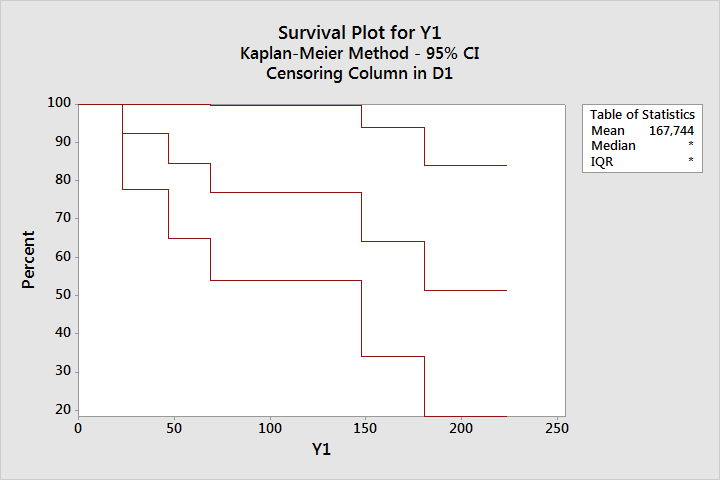
\includegraphics[scale=0.75]{Rhatt1.png}
\caption{A figure showing the survival data together with the 95 \% confidence interval.  }
\label{rhatt}
\end{figure}
\end{center}

The estimated lifetime $E(T_1) = \int \limits_{0}^{\infty} R(t)dt$ can be approximated by a sum when we use $\hat{R}_1(t) $ instead of $R_1(t)$. We the get\\
\begin{center}
 $  \hat{E(t)} \sum \limits_{i} \hat{R}(T_i)(T_i-T_{i-1}) =1\cdot (23-0)+0.9231\cdot (47-23)+ 0.8461\cdot (69-47)+0.7692\cdot (148-69)+0.6410\cdot (181-148)+0.5128\cdot (224-181)=  167.74 $
 \end{center}
This is the same as the area under the curve in figure \ref{rhatt}. \\
 
Because of censoring we do not have the last points, but if we pretend that the fail-rate continue as it has, the estimated expected lifetime could seem to be a little pessimistic. We also see that about half the population has failed at about 175. So I would expect the real value to be a bit higher than the estimation.


\section*{b)}
The Nelson-Aalen estimator is given by $$ \hat{Z}_{NA}(t) = \sum \limits_{T_{1_i} \leq t} \frac{d_i}{n_i} $$
With $d_i$ and $ n_i$ as in a). Nelson-Aalen values for the hazard rate is given in table \ref{NA}.
 

\begin{center}
\begin{table}[h!]
\centering
\begin{tabular}{ c l c r }
	& & & \\
	time & expression & & value \\ & & \\
23	&$ \frac{1}{13} $ & = & $ 0.0769 $\\ & & \\
47	&$ \frac{1}{13}+\frac{1}{12} $ & = & $ 0.1603 $\\ & & \\
69	&$ \frac{1}{13}+\frac{1}{12}+\frac{1}{11} $ & = & $0.2512$ \\ & & \\
148	&$ \frac{1}{13}+\frac{1}{12}+\frac{1}{11}+\frac{1}{6} $ & = & $ 0.4178 $ \\ & & \\
181 &$ \frac{1}{13}+\frac{1}{12}+\frac{1}{11}+\frac{1}{6}+\frac{1}{5} $ & = & $ 0.6178 $\\
   & & \\
\end{tabular}
\caption{Table with hazard rates calculated using the Nelson-Aalen estimator using the negatively stained data.}
\label{NA}
\end{table}
\end{center}

\begin{center}
\begin{figure}[h!]
\centering
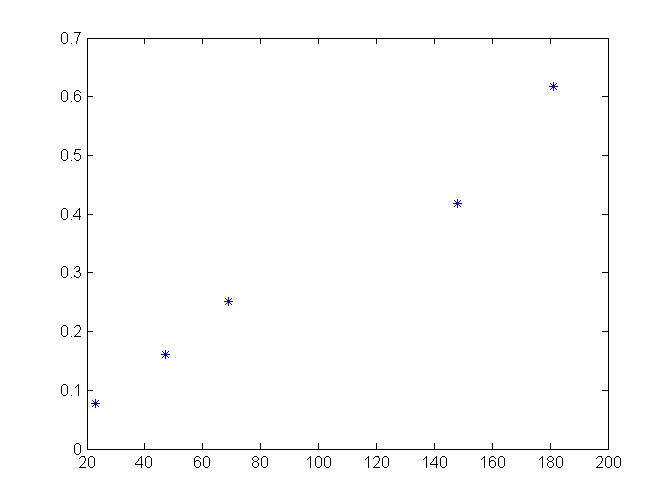
\includegraphics[scale=0.50]{NA}
\caption{Plot of Nelson-Aalen hazard-rate in table \ref{NA}, from the negatively stained data.  }
\label{NAh}
\end{figure}
\end{center}
From figure \ref{NAh} I would expect the hazard-rate to be constant, or close to constant, but it is difficult to be sure with so few data points.

\begin{center}
\begin{figure}[h!]
\centering
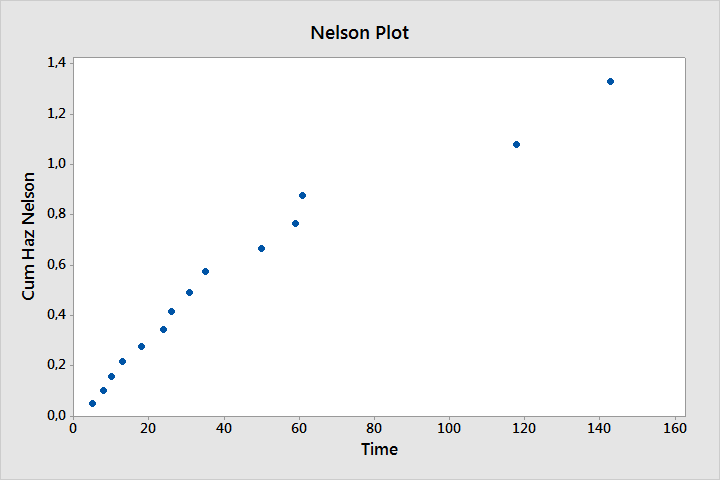
\includegraphics[scale=0.75]{nelson2.png}
\caption{Plot of Nelson-Aalen hazard-rate of the positively stained data from minitab.  }
\label{NAm}
\end{figure}
\end{center}

The hazard-rate in plot \ref{NAm} is not as straight as in plot \ref{NAh}. So the hazard-rate for the positively stained case could definitely be time-dependant. It seams to be concave shaped, so it has a decreasing failure rate. 

\section*{c)}

TTT plot is given by $$ (\frac{i}{n}, \frac{Y_i}{Y_n}) $$
Where $Y_i = \sum \limits_{j = 1}^{i-1} T_j + (n-i+1)T_i  $ 

\begin{center}
\begin{table}[h!]
\centering
\begin{tabular}{ c l c r }

	i/n &  & & $Y_i$\\
0.2	& $5\cdot 23 $ & = & $ 115 $\\
0.4	&$ 23+4\cdot47 $ & = & $ 211 $\\
0.6	&$ 23+47+3\cdot69 $ & = & $277$ \\
0.8	&$ 23+47+69+2\cdot148 $ & = & $ 435 $ \\
1.0 &$ 23+47+69+148+181 $ & = & $ 468 $\\
\end{tabular}
\caption{A table of the values used for the TTT-plot.}
\label{TTTt}
\end{table}
\end{center}

\begin{center}
\begin{figure}[h!]
\centering
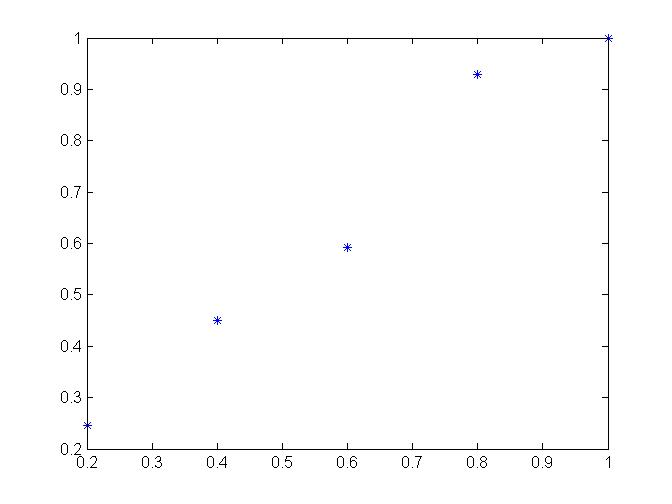
\includegraphics[scale=0.50]{TTT1}
\caption{TTT-plot made from the values in table \ref{TTTt}.}
\label{TTTh}
\end{figure}
\end{center}


We now want to test if the data has a monotone hazard-rate. To check this we can use a Barlow-Proschan's test:\\
$H_0 : T ~ \text{expon}(\lambda) $ versus $ H_1 : T $ has monotone hazard.

We the need to compute \\
$$ Z = \frac{W-\frac{n-1}{2}}{\sqrt{\frac{n-1}{2}}} $$ \\
where $$W = \frac{Y_1}{Y_n}+\frac{Y_2}{Y_n}+\cdots+\frac{Y_{n-1}}{Y_n}$$ where $Y_i$ is a above.
Reject $ H_1 $ if $ Z \leq -z_{\alpha/2} $ or $ Z \geq z_{\alpha/2} $. Barlow-Proschan's test only works with uncensored data, we therefore take out all censored data from the set before we do the calculations. 
This gives the following numbers:
$ n=5 $, $ W =2.2179  $, which gives $ Z = 0.1541 $. Therefore we easily reject $ H_1$ when $\alpha =0.05$. That is, when $ z_{\alpha/2} = 1.96 $, and conclude that the data does not have a monotone hazard-rate.\\

\begin{center}
\begin{figure}[h!]
\centering
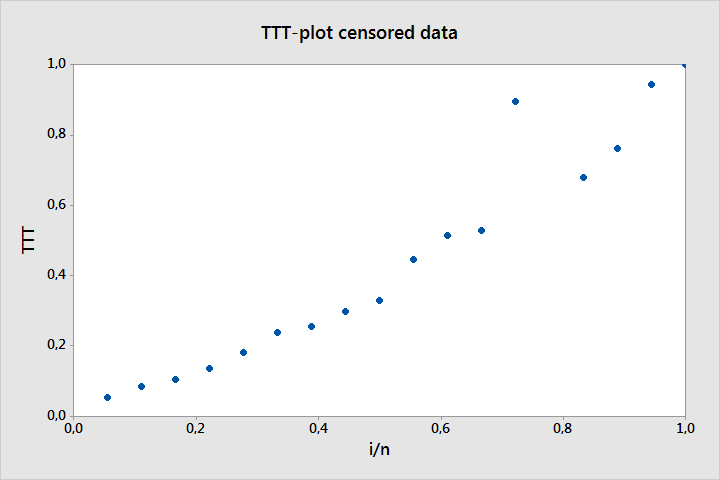
\includegraphics[scale=0.75]{TTT2.png}
\caption{TTT-plot by minitab of the positively stained data.}
\end{figure}
\end{center}

We now want to do a Barlow-Proschan-test for the positively stained data, because it looks like it might have some DFR-tendencies. As with in the negatively stained case we also here take away the censored data, and make a test with\\
$H_0 : T ~ \text{expon}(\lambda) $ versus $ H_1 : T $ has DFR.\\
We reject $H_1$ if $ Z\leq -z_\alpha $. Minitab gives $ n=18 $ $ W = 7.4858 $,  which gives a $Z = -0.1193 $. With $ z_{0.05} = 1.65 $, we do not reject $H_1 $ and conclude that the data for the positively stained case has DFR.\\

\section*{d)}
     
\begin{center}
\begin{figure}[h!]
\centering
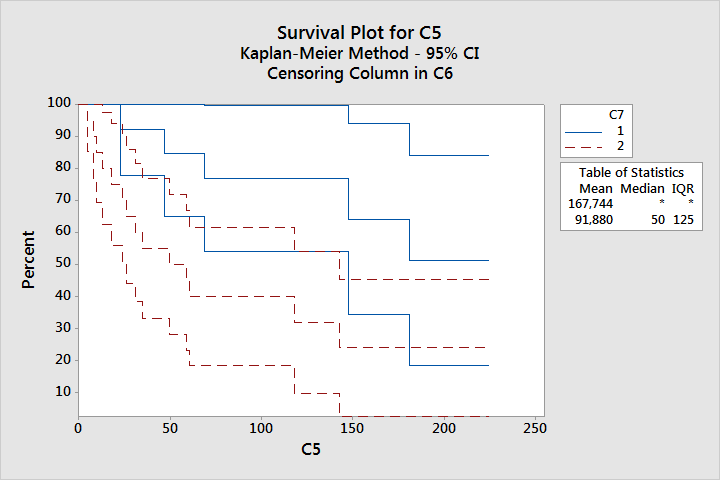
\includegraphics[scale=0.75]{same.png}
\caption{A survival plot with the negatively stained data(blue) and the positively stained data(red), by minitab.}
\label{same}
\end{figure}
\end{center}
As we can see in figure \ref{same} it seems that the population the negatively stained group had a tendency to live longer than the population in the positively stained group.

\section*{e)}
We want to test the data in d) to see if the groups really have a different lifetime using a logrank test. \\
$H_0 : R_1(t)=R_2(t) $ versus $ H_1 : R_1(t) \neq R_2(t) $.\\ We reject $H_0$ if $V \geq \chi^2_1 $. Where $V = \frac{(O_1-E_1)^2}{E_1}+\frac{(O_2-E_2)^2}{E_2} $, $E_i = \sum_{j=1}^k E_{i j} = \sum_{j=1}^k \frac{O_j}{N_j} \cdot N_{i j}$ is the estimated expected number of failures, $ O_j = \sum_{i=1}^n O_{i j}$ observed number of failures at time $T_j$, $N_j = \sum_{i=1}^n N_{i j}$ is the number at risk, $n$ is number of groups to compare, and $k$ is the number of failure times.\\
For this case $n =2$, $k = 19$. The rest of the numbers are given in the table \ref{V}. 

%\begin{center}
%\begin{table}[h!]
%\centering
%\begin{tabular}{ l c r }
%
%   & Group 1 & Group 2 \\
%  E & 9.77 & 9.23 \\
%  O & 5 & 14 \\
%
%\end{tabular}
%  \caption{Values used for calculating V.}
%  \label{V}
%\end{table}
%\end{center}

\begin{center}
\begin{table}[h!]
\centering
\begin{tabular}{ l c c c c c c c }

 Time & $O_{1 j}$ & $O_{2 j}$ & $N_{1 j}$ & $N_{2 j}$ & $N_{j}$ & $E_{1 j}$ & $ E_{2 j} $ \\
  5 & 0 & 1 & 13 & 20 & 33 & 13/33 & 20/33\\
  8 & 0 & 1 & 13 & 19 & 32 & 13/32 & 19/32\\
 10 & 0 & 1 & 13 & 18 & 31 & 13/31 & 18/31\\
 13 & 0 & 1 & 13 & 17 & 30 & 13/30 & 17/30\\
 18 & 0 & 1 & 13 & 16 & 29 & 13/29 & 16/29\\
 23 & 1 & 0 & 13 & 15 & 28 & 13/28 & 15/28\\
 24 & 0 & 1 & 12 & 15 & 27 & 12/27 & 15/27\\
 26 & 0 & 1 & 12 & 14 & 26 & 12/26 & 14/26\\
 31 & 0 & 1 & 12 & 13 & 25 & 12/25 & 13/25\\
 35 & 0 & 1 & 12 & 12 & 24 & 12/24 & 12/24\\
 47 & 1 & 0 & 12 & 11 & 23 & 12/23 & 11/23\\
 50 & 0 & 1 & 11 & 11 & 22 & 11/22 & 11/12\\
 59 & 0 & 1 & 11 & 10 & 21 & 11/21 & 10/21\\
 61 & 0 & 1 & 11 &  9 & 20 & 11/20 &  9/20\\
 69 & 1 & 0 & 11 &  8 & 19 & 11/19 &  8/19\\
118 & 0 & 1 &  6 &  5 & 11 & 6/11  &  5/11\\
143 & 0 & 1 &  6 &  4 & 10 & 6/10  &  4/10\\
148 & 1 & 0 &  6 &  3 & 9  & 6/9   &   3/9\\
181 & 1 & 0 &  5 &  1 & 6  & 5/6   &   1/6\\

% \hline
 \hline
 SUM & 5 & 14 & & & & 9.77 & 9.23
\end{tabular}
  \caption{Calculated values for $E_i$, $N_{i j}$, $O_{i j}$}
  \label{V}
\end{table}
\end{center}



We get $V = 4.7940 $. $\chi^2_1=3.84$ for $\alpha = 0.05$, so we reject the $H_0$ at $ \alpha = 0.05 $. We therefore conclude that the lifetimes are different.

\section*{f)}

\begin{center}
\begin{figure}[h!]
\centering
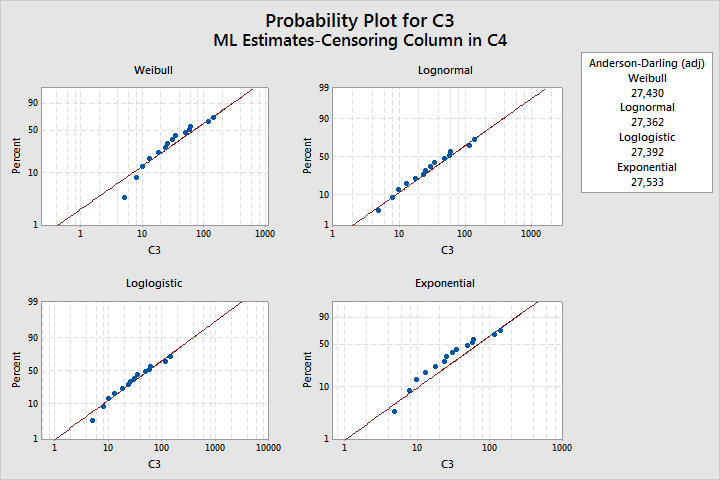
\includegraphics[scale=0.75]{pos.png}
\caption{Fitted distributions over the positively stained case.}
\label{pos}
\end{figure}
\end{center}
At figure \ref{pos} we see that the positively stained data fits the lognormal plot best. 



\begin{center}
\begin{figure}[h!]
\centering
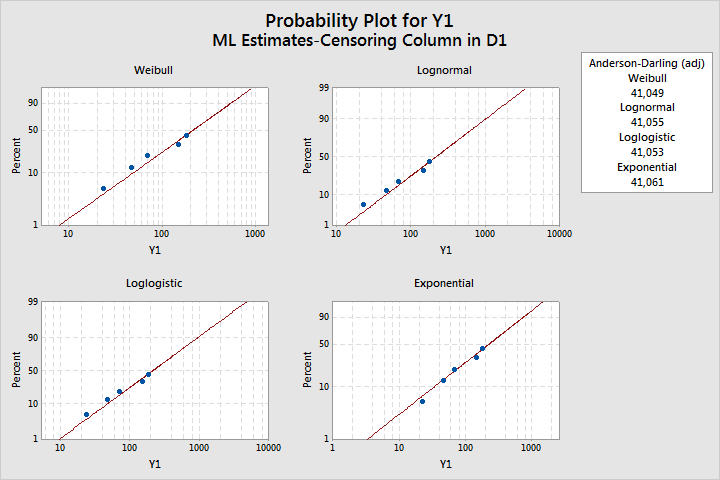
\includegraphics[scale=0.75]{neg.png}
\caption{Fitted distributions over the negatively stained case.}
\label{neg}
\end{figure}
\end{center}

At figure \ref{neg} we see that the data fits all the models, probably due to too little data, but if I had to, I would say log-logistics fits the data best.\\

The difference in the average lifetimes (MTTF) for the different models can be due of the different way the model fit data. Some models have a long tail, and some data have a higher peak at the center, changing the mean.

\section*{g)}
Log-location-scale families are distributions where $ Y = \ln(T) = \mu + \sigma Z $, Where $ Z $ is normal distributed.
The location parameter is the expected value, $\mu$. The location of the peak can be moved by changing $\mu$. The scale parameter, $\sigma$ determines the shape of the distribution. Changing $\sigma$ will spread or gather the probability.\\

To find the hazard-function for the log-logistics distribution we start with probability density function $ \phi(x) = \frac{e^{x}}{(e^{x}+1)^2} $, and the cumulative distribution function $ \Phi(x) = \frac{e^{x}}{e^{x}+1} $. From this we can calculate the survival-function, $ R(t) $.
$$ R(t) = P(T > t)= P(\ln(T) > \ln(t)) = P(\mu+\sigma Z > \ln t) = P(Z> \frac{\ln(t)-\mu}{\sigma}) = 1-\Phi(\frac{\ln(t)-\mu}{\sigma}) $$
so the survival function becomes
$$ R(t) = \frac{1}{e^{\frac{\ln(t)-\mu}{\sigma}}+1} $$
We also have $ f(t) = -R'(t) $, and with some work we get
$$f(t) =  \frac{e^{\frac{\ln(t)-\mu}{\sigma}}}{(e^{\frac{\ln(t)-\mu}{\sigma}}+1)^2} \cdot \frac{1}{t \sigma} $$
Finally we know that
$$ z(t) = \frac{f(t)}{R(t)} = \frac{e^{\frac{\ln(t)-\mu}{\sigma}}}{e^{\frac{\ln(t)-\mu}{\sigma}}+1}\frac{1}{t \sigma} = \frac{1}{\sigma} \frac{t^{1/\sigma-1}}{t^{1/\sigma}+e^{\mu/\sigma}} $$
Which is the hazard distribution for the log-logistics distribution.

\end{document}